\documentclass[en]{university}

\faculty{Department of Computer Engineering}
\course{Artificial Intelligence}
\subject{Mini Project 3 Theory Questions}
\professor{Dr. Rohban}
\student{Parsa Mohammadian}

\begin{document}

\setupdocument

\section{}

\subsection{}

We decide if a move violates game rules or not by using d-separation algroithm to find out 
if A and B are still independent. A valid move for each of the graphs is illustrated in 
figure \ref{fig:validmoves}.

\begin{figure}
    \centering
    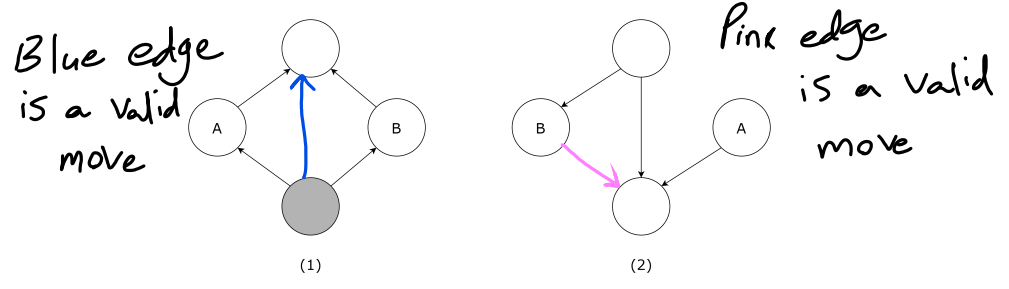
\includegraphics[width=0.8\textwidth]{assets/1-a.png}
    \caption{Valid Moves}
    \label{fig:validmoves}
\end{figure}

\subsection{}

\section{}

base factor headers are:

\begin{align*}
    A : \begin{bmatrix}
        A & C & D & P(A | C, D)
    \end{bmatrix} \\
    B : \begin{bmatrix}
        B & D & E & G & P(B | D, E, G)
    \end{bmatrix} \\
    C : \begin{bmatrix}
        C & F & I & P(C | F, I)
    \end{bmatrix} \\
    D : \begin{bmatrix}
        D & G & H & P(D | G, H)
    \end{bmatrix} \\
    E : \begin{bmatrix}
        E & P(E)
    \end{bmatrix} \\
    F : \begin{bmatrix}
        F & H & P(F | H)
    \end{bmatrix} \\
    G : \begin{bmatrix}
        G & H & P(G | H)
    \end{bmatrix} \\
    H : \begin{bmatrix}
        H & I & P(H | I)
    \end{bmatrix} \\
    I : \begin{bmatrix}
        I & P(I)
    \end{bmatrix}
\end{align*}

\subsection{B, E, D, C, H, I}

\begin{align*}
    \text{Join} (B, D, E, G)  \rightarrow \text{Eliminate} (B) : \begin{bmatrix}
        D & E & G & P(D, E, G)
    \end{bmatrix} \\
    \text{Join} (\text{Current}, E) \rightarrow \text{Eliminate} (E) : \begin{bmatrix}
        D & G & P(D, G)
    \end{bmatrix} \\
    \text{Join} () \rightarrow \text{Eliminate} D : \begin{bmatrix}
        G & P(G)
    \end{bmatrix}
\end{align*}

\subsection{I, H, C, D, E, B}

\end{document}